\chapter{Supplemental Material for Chapter \ref{chap:Proof of concept method to identify enhancers}}

%%%%%%%%%%%%%%%%%%%%%%%%%%%%%%%%%%%%%%%%%%%%%%%%%%%%%%%%%%%%%%%%%%%%%%%%%%%%%%%%
\section{Supplementary Figures}
%%%%%%%%%%%%%%%%%%%%%%%%%%%%%%%%%%%%%%%%%%%%%%%%%%%%%%%%%%%%%%%%%%%%%%%%%%%%%%%%

\begin{figure}[h]
    \centering
    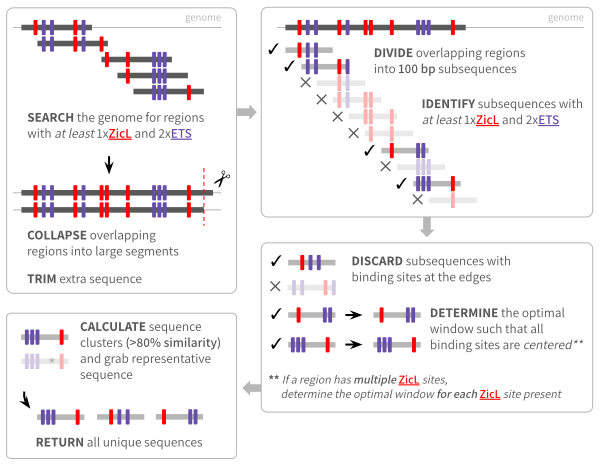
\includegraphics[scale=.5]{3_figures-and-files/FigS1_KYN-Search.png}
    \caption[KYN library search methodology]{\textbf{KYN library search methodology.} Schematic of the search methodology for identifying elements for the KYN library from the \textit{Ciona intestinalis type A} genome. First, the genome is scanned on a chromosome by chromosome basis for large genomic blocks containing at least one Zic site and two ETS binding sites. These genomic blocks are then collapsed upon each other based on overlapping coordinates and trimmed. Then, 100 bp subsequences are extracted from the large genomic blocks and screened for if they have minimum at least one Zic site and two ETS binding sites. The subsequences are discarded if they have binding sites on the edge of the sequence, and all subsequences are modified such that all binding sites are centered within the 100 bp window. Finally, the sequence similarity is calculated between all 100 bp windows and all windows with less than 80\% similarity to each other as calculated by the hamming distance are included within the KYN library.}
    \label{fig:supplement kyn library search}
\end{figure}